\section{Related Work}

It is a nontrivial task to visualize multiclass data on density maps and various designs have been used. The Class Buffer model unifies those various designs into a single model~\cite{jo2019declarative}.

\begin{figure}
	\centering
	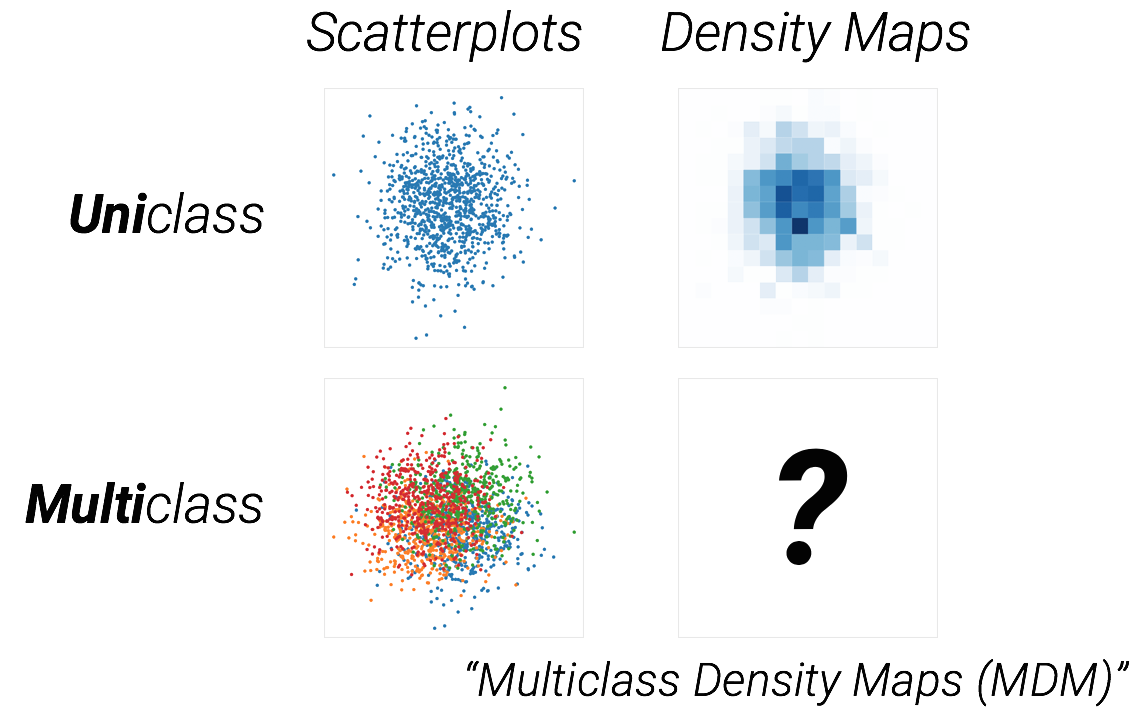
\includegraphics[width=\columnwidth]{./figures/motivation}
	\caption[motivation]{Scatterplots show two dimensional data with no additional property. These are called uniclass scatterplots (top left). When the scatterplot is extended with multiple classes it becomes a multiclass scatterplot (bottom left). Instead of single points to represent data points, these values can be aggregated and displayed in a way that indicates higher concentrations with i.e. darker colors (top right). An important task remains to show multiple classes with these density maps. These kind of maps are multiclass density maps.\\\textcopyright~Jaemin Jo, [Online; accessed June 04., 2019] \url{https://raw.githubusercontent.com/e-/Multiclass-Density-Maps/master/motivation.png} - BSD-2-Clause}~\label{fig:motivation}
\end{figure}

With more data to show, the separation of classes, perception of clusters and even just the basic comprehension becomes an ever-growing problem~\cite{jo2019declarative}. Scatterplots as well as density maps additionally have a fundamental drawback: they're ineligible for retrieving rates or numbers from the map. For example, few people will have the time or ambition to count hundreds (or thousands) of dots in order to know the precise number represented. They'll likely know that some places have "more" of what is shown than others, but they won't know necessarily by how much. The same principle applies to density maps where it is not easy for viewers to tell what color in a region represents how much data.
When dealing with multiclass density maps different obstacles come to hand that limit the readability and comprehensibility of the data that is shown in the plot.
As soon as the number of data points increases, multiclass maps must resort to dimension reduction (DR) or visual encoding (VE) techniques to remain readable. Multiclass Density Maps use multiple overlaying density maps, derived from scatterplots, to display data in a way that the comprehension of the data can be improved~\cite{jo2019declarative}.

Scatterplots have been used for almost two centuries as a way to visually represent data~\cite{friendly2005early}. Much of their popularity has been due to their ability to allow correlations to be easily perceived by a human viewer~\cite{cleveland1993visualizing, harris2000information}. Multiclass scatterplots contain higher dimensional data and hence have to be designed more carefully.
When it comes to density maps the data can be masked or mixed, among other visual enhancements. This process might hide or obfuscate data from being perceived fast. The viewer consequently might has to engage in greater cognitive effort to understand what is depicted.

The problem of scaling the visualization, either by adding or by filtering information via aggregation or binning, has been addressed in various articles~\cite{cottam2013overplotting, cottam2014abstract, mayorga2013splatterplots, wickham2013bin}. From this work three facets can be identified for scalability:

\begin{itemize}[leftmargin=*]
	\setlength\itemsep{0.1em}
	\item \textbf{data size} related to the number of data points and categories,
	\item \textbf{perceptual processing} related to the ability to perform some tasks efficiently given a data size, and
	\item \textbf{computation speed} related to the time to compute an image from a visualization technique given a data size.
\end{itemize}

Visualization techniques should be versatile, support large data sizes and be easy to understand, all while performing important perceptual tasks quickly. Interactive exploration can be facilitated by fast reaction and computation times. The type of interaction influences the time a user may wait for the plot to be refreshed~\cite{miller1968response, shneiderman1984response}, ranging from 25 milliseconds up to 10 seconds.
Managing large data sizes while allowing effective perceptual processing is already a challenge, and the goal of the Class Buffer model is to design a model that can improve all the three facets of scalability~\cite{jo2019declarative}.

% \textcolor{red}{
% 	Duis autem vel eum iriure dolor in hendrerit in vulputate velit esse molestie consequat, vel illum dolore eu feugiat nulla facilisis at vero eros et accumsan et iusto odio dignissim qui blandit praesent luptatum zzril delenit augue duis dolore te feugait nulla facilisi. Lorem ipsum dolor sit amet, consectetuer adipiscing elit, sed diam nonummy nibh euismod tincidunt ut laoreet dolore magna aliquam erat volutpat.}

% \textcolor{red}{
% 	Ut wisi enim ad minim veniam, quis nostrud exerci tation ullamcorper suscipit lobortis nisl ut aliquip ex ea commodo consequat. Duis autem vel eum iriure dolor in hendrerit in vulputate velit esse}

% \textcolor{red}{
% 	Lorem ipsum dolor sit amet, consetetur sadipscing elitr, sed diam nonumy eirmod tempor invidunt ut labore et dolore magna aliquyam erat, sed diam voluptua. At vero eos et accusam et justo duo dolores et ea rebum. Stet clita kasd gubergren, no sea takimata sanctus est Lorem ipsum dolor sit amet. Lorem ipsum dolor sit amet, consetetur sadipscing elitr, sed diam nonumy eirmod tempor invidunt ut labore et dolore magna aliquyam erat, sed diam voluptua. At vero eos et accusam et justo duo dolores et ea rebum. Stet clita kasd gubergren, no sea takimata sanctus est Lorem ipsum dolor sit amet. Lorem ipsum dolor sit amet, consetetur sadipscing elitr, sed diam nonumy eirmod tempor invidunt ut labore et dolore magna aliquyam erat, sed diam voluptua. At vero eos et accusam et justo duo dolores et ea rebum. Stet clita kasd gubergren, no sea takimata sanctus est Lorem ipsum dolor sit amet.}

% \textcolor{red}{
% 	Duis autem vel eum iriure dolor in hendrerit in vulputate velit esse molestie consequat, vel illum dolore eu feugiat nulla facilisis at vero eros et accumsan et iusto odio dignissim qui blandit praesent luptatum zzril delenit augue duis dolore te feugait nulla facilisi. Lorem ipsum dolor sit amet, consectetuer adipiscing elit, sed diam nonummy nibh euismod tincidunt ut laoreet dolore magna aliquam erat volutpat.}
